\documentclass[uplatex,dvipdfmx,a4paper,10pt]{jsarticle}

\usepackage{amsmath,amsthm,amssymb}
\usepackage[dvipdfmx]{graphicx}
\usepackage{bm}
\usepackage{ascmac}
%
\usepackage{multirow}
\usepackage{wrapfig}

\usepackage{xcolor}

\usepackage{textcomp}

\usepackage[dvipdfmx]{hyperref}
\usepackage{pxjahyper}

%
\pagestyle{empty}
%% 高さの設定
\usepackage{geometry}
\geometry{left=25truemm, right=25truemm, top=25truemm, bottom=25truemm}

%
\abovecaptionskip=-1pt
%\belowcaptionskip=-1pt
%
\renewcommand{\baselinestretch}{0.85} % 全体の行間調整
\renewcommand{\figurename}{Fig.}
\renewcommand{\tablename}{Tab.}
%
\makeatletter 
\def\section{\@startsection {section}{1}{\z@}{1.5 ex plus 2ex minus -.2ex}{0.5 ex plus .2ex}{\large\bf}}
\def\subsection{\@startsection{subsection}{2}{\z@}{0.2\Cvs \@plus.5\Cdp \@minus.2\Cdp}{0.1\Cvs \@plus.3\Cdp}{\reset@font\normalsize\bfseries}}
\makeatother 
%
\graphicspath{{../fig/peak_bunri/}}
%
\title{ピーク分離(ベースライン補正)に関するメモ}
% \subtitle{ポリカーボネートの降伏挙動とエンタルピー緩和}
\author{東亞合成 佐々木裕}
\date{\today}

\begin{document}

\maketitle

% \begin{wrapfigure}{r}{0.4\textwidth} %% 図右寄せの場合{r}
% 	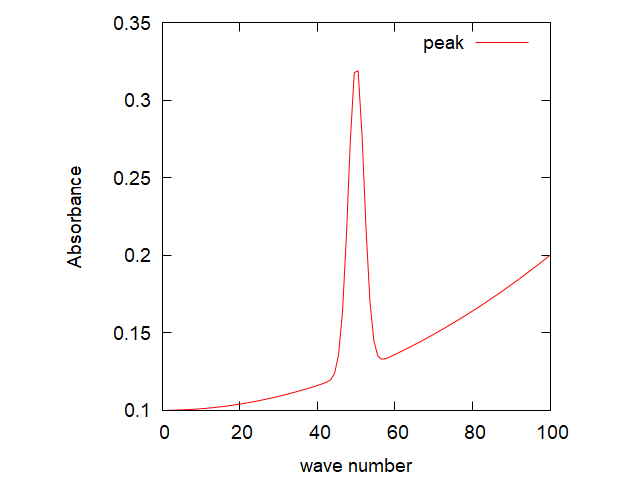
\includegraphics[width=0.4\textwidth]{peaks.png}
% 	\caption{一般的な吸収曲線}
% 	\label{fig1}
% \end{wrapfigure}

\section{やりたいこと}

赤外(Infra Red: IR)や近赤外(Near Infra Red: NIR)を用いた分光スペクトルは非常に多くの吸収バンドで構成されるため、ピークどうしの重なりが生じます。
Fig.\ref{fig1} に単一の吸収ピークが一般にベースラインと呼ばれる非常に幅広い吸収と重なった場合の例を示しました。

このメモでは、ベースライン補正について簡単にまとめます\footnote{
    このメモは、\href{https://www.perkinelmer.co.jp/tabid/2468/Default.aspx}{PerkinElmer 社のテクニカルサポートのサイト}を参考にして、簡略化して再構築したものです。

    このサイトによれば、以下の2つの文献が参考資料としてあげられています。
    \begin{enumerate}
        \item \href{https://onlinelibrary.wiley.com/doi/abs/10.1002/anie.197807853}{G. Talsky, L. Mayring, and H. Kreuzer, Angew. Chem., Int. Ed. m., 11, 785 (1978)}
        \item \href{https://www.tandfonline.com/doi/abs/10.1080/05704928508060434}{Dixit L, Ram. S, Applied Spectroscopy Reviews, 21, (4), 311–418 (1985)}
    \end{enumerate}
}。

\section{考え方}

\subsection{赤外分光法とは}
まず、赤外分光法について簡単に振り返りましょう。
赤分光法は、物質に赤外光を照射し、透過または反射した光を測定することで、試料の構造解析や定量を行う分析手法です。

赤外光は、分子中の官能基の振動や回転運動に基づき吸収されます。
分子の振動や回転の状態を変化させるのに必要なエネルギー(赤外光の波長)は、物質の化学構造によって異なります。
従って、物質に吸収された赤外光を測定すれば、化学構造や状態に関する情報を得ることができます。

赤外吸収においては、特定の官能基に対応する特性吸収は輝線のような単一のエネルギーに対応する吸収ではなく、その官能基が置かれた微小な空間的な状態に応じてその励起寿命が影響されるため、一般に、吸収によるスペクトル形状はガウス分布とローレンツ分布の両方の特徴を有することが知られています。
そして、その吸収される光量子量は注目する官能基のモル濃度に比例すると考えます。

% \begin{wrapfigure}{r}{0.4\textwidth} %% 図右寄せの場合{r}
% 	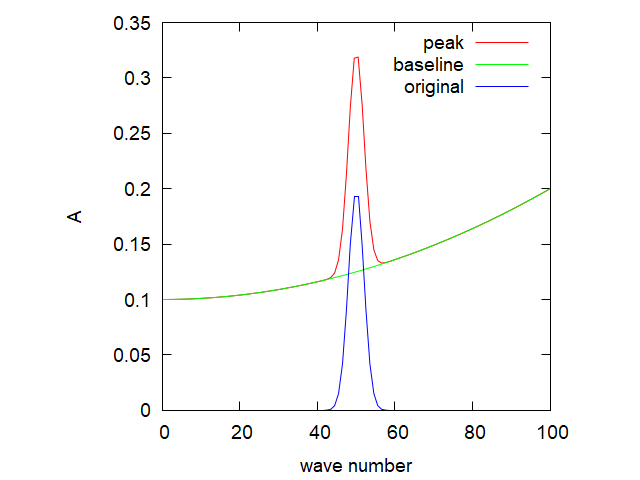
\includegraphics[width=0.4\textwidth]{peaks_lc.png}
% 	\caption{線形結合での近似}
% 	\label{fig2}
% \end{wrapfigure}

\begin{figure}[bt]
    \begin{minipage}{0.5\hsize}
        \begin{center}
        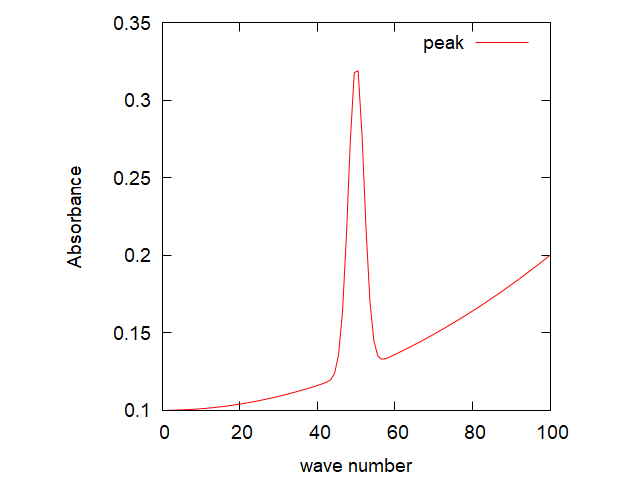
\includegraphics[width=.8\textwidth]{peaks.png}
        \caption{一般的な吸収曲線}
        \label{fig1}
        \end{center}
    \end{minipage}
    \begin{minipage}{0.5\hsize}
        \begin{center}
        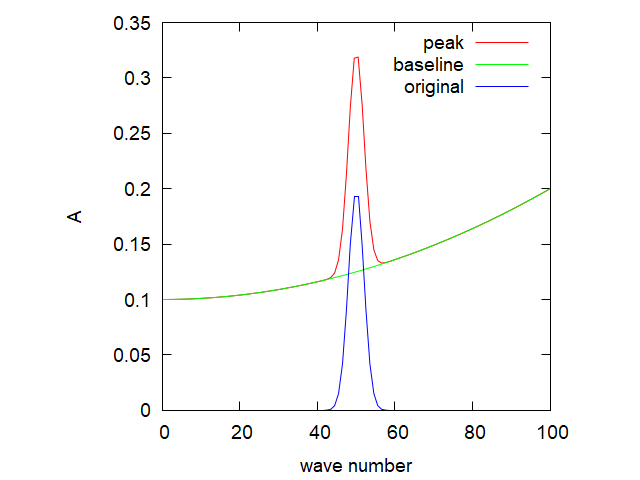
\includegraphics[width=.8\textwidth]{peaks_lc.png}
        \caption{線形結合での近似}
        \label{fig2}
        \end{center}
    \end{minipage}
\end{figure}

\subsection{対象の簡略化}
まず、今回対象とする分光吸収スペクトルを波長 $\lambda$ の関数として $A(\lambda)$ と表し、これが、注目する吸収ピークを表す分布関数 $f(\lambda)$ と、ベースラインを表す $g(\lambda)$ との線形結合の形で以下のように近似できるとしましょう。
\begin{align*}
    A(\lambda) = f(\lambda) + g(\lambda)
\end{align*}

ここで、特性吸収をガウス分布で、ベースラインを二次関数で以下のように近似した場合の吸収スペクトルを、Fig \ref{fig2} に示しました。

具体的には以下のように設定したものであり、
\begin{align*}
f(\lambda) &= \dfrac{1}{\sqrt{2 \pi} s} exp \left[\dfrac{-(\lambda-p)^2}{2s^2}\right] \\
g(\lambda) &= a\lambda^2 + C \\
where:& p=50, s= 2, a=1e-5, C=0.1
\end{align*}
$p$ がピークトップの位置、$s$ がガウス分布の標準偏差(スペクトル幅と相関)に対応します。



\subsection{ピークの微分}

% \begin{wrapfigure}{r}{0.4\textwidth}
% 	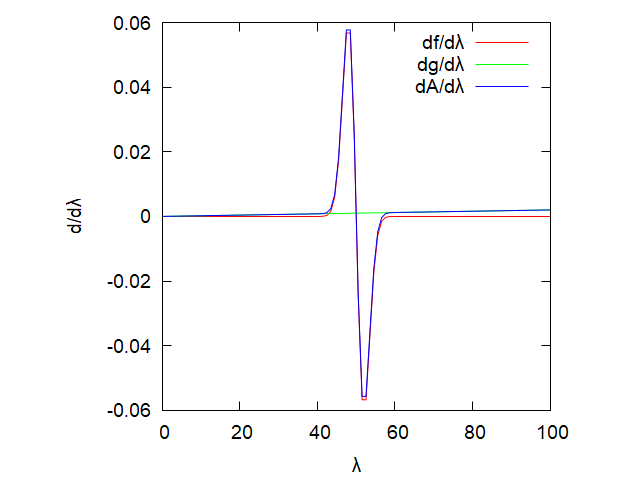
\includegraphics[width=0.4\textwidth]{der_1.png}
% 	\caption{近似した吸収スペクトルの一階微分}
% 	\label{fig3}
% \end{wrapfigure}

前述のようなベースラインのシフトを含む吸収スペクトルからベースライン補正を行うことを考えます。

具体的には、以下に示した和の微分の公式を利用して、それぞれの関数の微分の和の形にして考えていきます。
\begin{align*}
    \dfrac{\mathrm{d}(f+g)}{\mathrm{d} \lambda} = \dfrac{\mathrm{d}f}{\mathrm{d} \lambda} + \dfrac{\mathrm{d}g}{\mathrm{d} \lambda}
\end{align*}

今回の近似した吸収スペクトルでは以下のように微分され、それらの和と合わせてプロットすると Fig. \ref{fig3} となります。
\begin{align*}
    \dfrac{\mathrm{d}(f)}{\mathrm{d} \lambda} &= \dfrac{-\lambda}{\sqrt{2 \pi} s^3} exp \left[\dfrac{-(\lambda-p)^2}{2s^2}\right] \\
    \dfrac{\mathrm{d}(g)}{\mathrm{d} \lambda} &= 2a\lambda \\
    where:& p=50, s= 2, a=1e-5
\end{align*}

% \begin{wrapfigure}{r}{0.4\textwidth}
% 	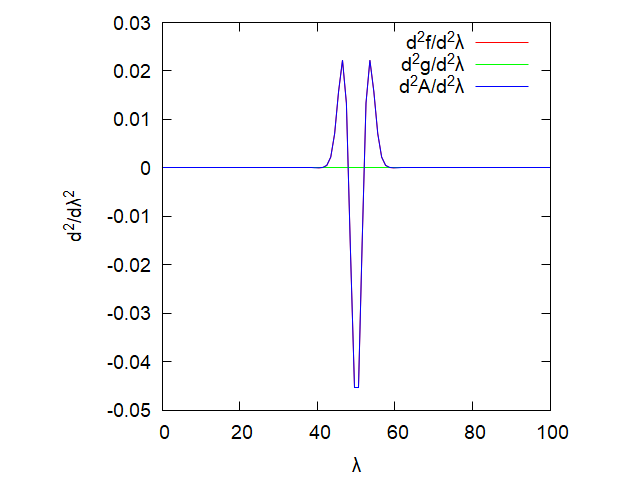
\includegraphics[width=0.4\textwidth]{der_2.png}
% 	\caption{近似した吸収スペクトルの二階微分}
% 	\label{fig4}
% \end{wrapfigure}

この式展開からも理解できるように、ベースラインの影響はかなり低減され、特性吸収に対してはプレファクタの$\dfrac{-\lambda}{\sqrt{2 \pi} s^3}$ によって、ピークトップとなる波長 $\lambda=p$ においてゼロ点と交わることが確認できます。

次に二階微分の場合を考えます。
\begin{align*}
    \dfrac{\mathrm{d}^2 f}{\mathrm{d} \lambda^2} &= \dfrac{1}{\sqrt{2 \pi} s^5} (\lambda^2 - s^2) exp \left[\dfrac{-(\lambda-p)^2}{2s^2}\right] \\
    \dfrac{\mathrm{d}^2 g}{\mathrm{d} \lambda^2} &= 2a \\
    where:& p=50, s= 2, a=1e-5
\end{align*}

これらの和と合わせてプロットすると Fig. \ref{fig4} となります。
\begin{figure}[hbt]
    \begin{minipage}{0.5\hsize}
        \begin{center}
        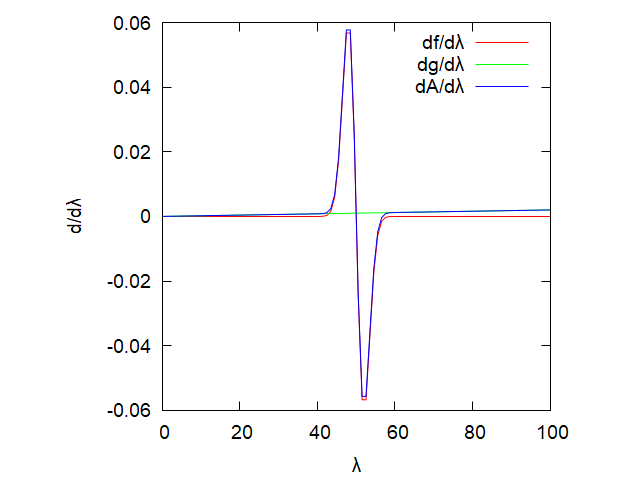
\includegraphics[width=.8\textwidth]{der_1.png}
        \caption{近似した吸収スペクトルの一階微分}
        \label{fig3}
        \end{center}
    \end{minipage}
    \begin{minipage}{0.5\hsize}
        \begin{center}
        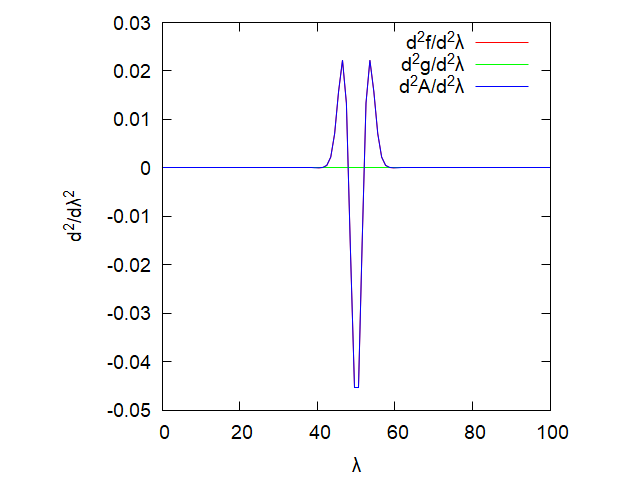
\includegraphics[width=.8\textwidth]{der_2.png}
        \caption{近似した吸収スペクトルの二階微分}
        \label{fig4}
        \end{center}
    \end{minipage}
\end{figure}

二階微分においては、(二次関数で近似した)ベースラインの影響は僅かな大きさの定数項となり、特性吸収は下に凸のピークとなります。
なお、このピークハイトの絶対値は微分前の値とは異なっていることに注意してください。

\subsection{ピークハイトの比較(定量性)}

\begin{wrapfigure}{r}{0.4\textwidth}
	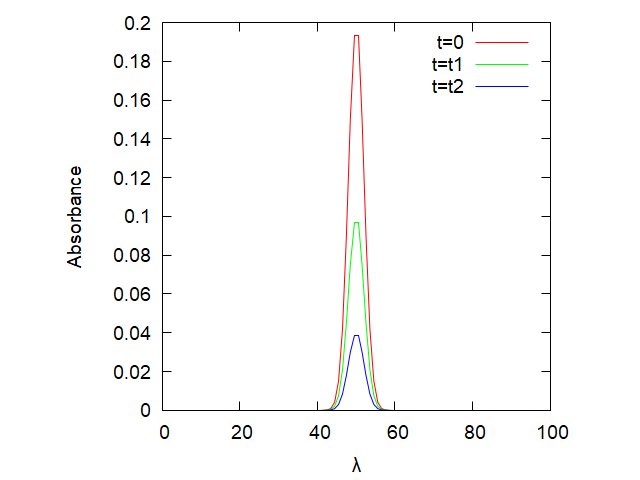
\includegraphics[width=0.4\textwidth]{peaks_multi.png}
	\caption{近吸収強度の異なるオリジナルスペクトル:測定者には見えない真の値}
	\label{fig5}
\end{wrapfigure}

前述のように、二階微分したピークハイトの大きさはプレファクタの影響によりオリジナルのそれとは異なっています。
しかしながら、「その吸収される光量子量は注目する官能基のモル濃度に比例する」という仮定が成立する範囲においては、同一の分布関数(スペクトル幅に対応する分散が同一)に基づいて吸収強度がモル濃度に比例することになります。

ここで、時間変化のトラジェクトリのように特定の官能基の濃度が時間変化する場合を考えましょう。
Fig. \ref{fig5} に、仮想的な「測定者では観測できない真のスペクトル変化」を示しました。
基準となる $t=0$ におけるピーク高さが、$t=t1$ で半分に、そして $t=t2$ で20\% になったものとしています。

実際の吸収スペクトルの観測では、上記の特性吸収にベースラインの影響が入りますし、測定状態に応じてベースラインの縦シフトも入ってスペクトル全体がずれてきます。
そのような状態をシミュレートしたものが、Fig.\ref{fig6} です。

このような条件下でも、二階微分を取ったスペクトルのトラジェクトリでのピークハイトを比として評価すれば Fig. \ref{fig7} のようになり、異なるサンプル間でのピークハイトの比の関係は微分の有無によらずに保たれることが確認できます。
\begin{figure}[htb]
    \begin{minipage}{0.5\hsize}
        \begin{center}
        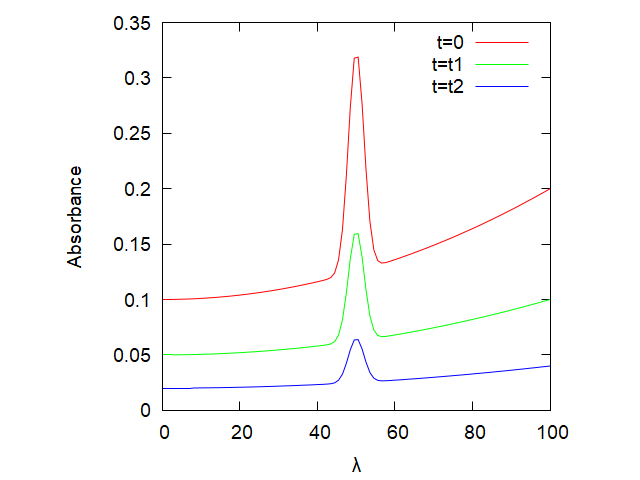
\includegraphics[width=.8\textwidth]{peaks_multi_shifted.png}
        \caption{ベースラインのドリフトも入った実測スペクトル}
        \label{fig6}
        \end{center}
    \end{minipage}
    \begin{minipage}{0.5\hsize}
        \begin{center}
        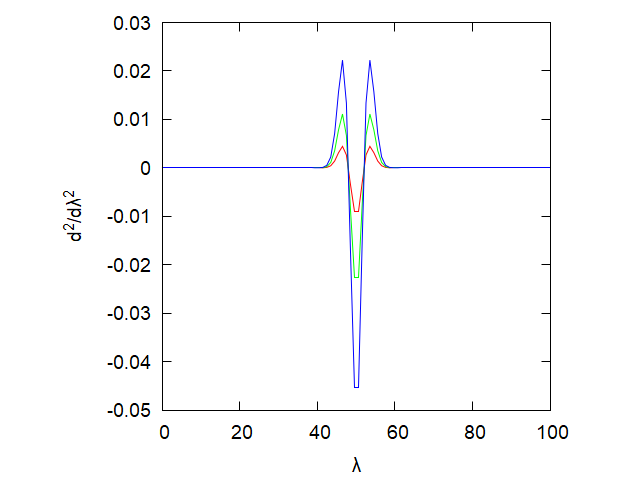
\includegraphics[width=.8\textwidth]{der_2_multi.png}
        \caption{左記を二階微分したスペクトル}
        \label{fig7}
        \end{center}
    \end{minipage}
\end{figure}

\subsection{注意点}

このメモでは、ベースラインのシフトのようにたかだか二次関数程度で記述できるものとの線形結合の形で吸収スペクトルを近似した場合のベースライン補正についての考え方を、図の例を上げながら説明を行いました。

しかしながら、この注目した吸収スペクトルの分散程度の波長の範囲において他の吸収ピークが共存して、そのピーク高さが注目するトラジェクトリ領域で同時に変化していた場合は、その影響を強く受けることになります。
周りの吸収に注意して、データ処理をすることを強くお勧めします。

\end{document}